%%%% FromHawking_DLIndaba2026.tex
\typeout{From Hawking to Intelligent Markets -- DL Indaba 2026}

\documentclass{article}
\pdfpagewidth=8.5in
\pdfpageheight=11in

\usepackage{ijcai26}
\usepackage{times}
\usepackage{soul}
\usepackage{url}
\usepackage[hidelinks]{hyperref}
\usepackage[utf8]{inputenc}
\usepackage[small]{caption}
\usepackage{graphicx}
\usepackage{amsmath}
\usepackage{amsthm}
\usepackage{booktabs}
\usepackage{algorithm}
\usepackage{algorithmic}
\usepackage{multirow}
\usepackage{enumitem}
\usepackage{xcolor}
\usepackage[switch]{lineno}

% Comment out for camera-ready
\linenumbers

% Enable subsubsection numbering (ijcai26.sty sets this to 2)
\setcounter{secnumdepth}{3}

\urlstyle{same}

\newtheorem{definition}{Definition}
\newtheorem{proposition}{Proposition}

\pdfinfo{
/TemplateVersion (IJCAI.2026.0)
}

\title{From Hawking to Intelligent Markets: Federated Market Analytics\\
and Optimized Spatial Retail Systems for Informal Economies in African Smart Cities}

\author{
Anonymous Authors
}

\begin{document}

\maketitle

\begin{abstract}
As African cities pursue smart city agendas, modern market initiatives seek to relocate street vendors into standardised hubs. While these policies target improved sanitation and urban order, they ignore the economic logic of subsistence-level retailers, primarily women and youth who rely on the high foot traffic generated by street hawking.
This misalignment creates an inclusion gap, like high entry barriers resulting from exorbitant rent fees, taxes, licenses, and reduced customer access, resulting into vendor displacement and a descent into poverty. This paper presents a dual-intervention framework.
First, we develop a federated learning system for distributed market intelligence that preserves vendor data sovereignty while also enabling collective demand--supply insights.
Second, we introduce AI-optimised modular retail units that address the economic and spatial barriers of traditional market infrastructure.
We formalise the \emph{inclusion gap} as the per-vendor economic penalty of lacking formal infrastructure, and derive digital demand-pull and risk-weighted allocation models.
Experiments on Rwanda's Establishment Census of 269,326 enterprises, where 87.8\% of these are informal, World Bank Enterprise Surveys, WFP market prices across Rwanda and Uganda, WorldPop density grids, and OpenStreetMap data demonstrate that:
(i)~federated formalization prediction achieves 98.6\% accuracy (FedAvg) and 100\% (FedProx) versus 87.5\% for isolated local models;
(ii)~modular units yield net vendor income with a 7.1$\times$ improvement;
(iii)~risk-weighted spatial allocation outperforms population-proportional placement under identical budgets.
A comparative Rwanda--Uganda benchmark on 629 market clients validates cross-border generalisability.
\end{abstract}

%=================================================================
\section{Introduction}
\label{sec:intro}
%=================================================================

Across sub-Saharan Africa, informal enterprises constitute the dominant economic form.
In Rwanda, the 2023 Establishment Census records 269,326 enterprises, of which 229,764 (87.8\%) operate informally \cite{nisr2023ec}.
A striking 92.2\% are micro-scale (1--3 workers), and 63.2\% hold capital below 300,000~RWF (\textasciitilde\$214).
Municipal smart city strategies, such as the Kigali Master Plan 2050 \cite{kigali2019master}, prescribe relocation into modern market halls with formalised rent, licensing, and sanitation standards.
However, annual rent in traditional modern markets reaches 1,200,000~RWF, compared with median informal turnover of only 250,000~RWF/year.
This rent-to-revenue mismatch makes formal markets \emph{economically unviable} for the overwhelming majority of informal vendors, creating what we term the \emph{inclusion gap}.

This paper makes three contributions:
\begin{enumerate}[label=\alph*)]
    \item Inclusion gap formalisation where we define a per-district metric quantifying the annual economic penalty vendors suffer from lacking formal market infrastructure, and extend it with how much digital infrastructure boosts vendor revenue through better demand matching (digital demand-pull coefficient) and the probability that a modular retail unit placed in that district will fail economically (viability risk score).
    \item Federated market intelligence where we deploy FedAvg \cite{mcmahan2017communication} and FedProx \cite{li2020federated} for two tasks: (a)~formalization prediction from enterprise survey features, and (b)~multi-commodity food price forecasting across 629 market-level clients in Rwanda and Uganda.
    \item \textbf{AI-Optimised Modular Retail Units.} We design a spatial allocation algorithm that distributes low-cost modular trading structures to maximise system-wide vendor viability under a fixed budget constraint.
\end{enumerate}

%=================================================================
\section{Related Work}
\label{sec:background}
%=================================================================

\subsection{Urban Informality and Forced Formalisation}

Street vending is the primary livelihood for over 2 billion workers globally, with informal employment accounting for 55--80\% of urban jobs in African cities \cite{ilo2023weso}.
Chen~\shortcite{chen2023rethinking} argues that informality is not a transitional phase but a structural feature of developing economies that requires integration rather than elimination.
Forced relocation policies, often termed ``clean-up'' or ``decongestion'' campaigns, have been documented across Johannesburg, Nairobi, Accra, and Kigali \cite{roever2023street}.
These interventions typically reduce vendor income by removing access to high-traffic locations while imposing unaffordable formal costs.
The COVID-19 pandemic further exposed the vulnerability of informal workers \cite{skinner2021covid}, with Adhikari and Shrestha~\shortcite{adhikari2023vendors} finding that post-pandemic recovery has been slowest for vendors displaced into formal markets.
Herrera and L\'{e}autier~\shortcite{herrera2023informal} demonstrate through spatial analysis that informality correlates strongly with urbanisation rate and infrastructure deficits across sub-Saharan Africa.

\subsection{Federated Learning for Resource-Constrained Settings}

Federated learning (FL) enables model training across distributed clients without centralising raw data \cite{mcmahan2017communication,kairouz2021advances}.
FedAvg aggregates locally trained model parameters via weighted averaging, while FedProx \cite{li2020federated} adds a proximal regularisation term to handle statistical heterogeneity.
Recent comprehensive surveys \cite{zhang2022fedsurvey,wen2023survey} identify data heterogeneity, communication efficiency, and privacy as key FL challenges, all of which are acute in informal market settings where vendors are privacy-sensitive and connectivity is intermittent.
Pfitzner et al.~\shortcite{pfitzner2021fedhealth} demonstrate FL's promise in healthcare settings with analogous privacy constraints, while Nguyen et al.~\shortcite{nguyen2022fliot} survey FL for resource-constrained IoT devices.
However, applications of FL to informal market systems in developing economies remain entirely unexplored.

\subsection{Digital Platforms and Spatial Market Design}

Digital platforms have shown promise in connecting informal micro-enterprises to broader markets.
Mobile money, which has reached over 1.75 billion registered accounts in sub-Saharan Africa \cite{suri2023fintech}, provides a ready digital layer for vendor transactions.
However, most digital platforms require centralised data collection that excludes privacy-conscious vendors.
Spatial allocation of market infrastructure has traditionally relied on population-proportional heuristics or maximal covering location models.
Osei et al.~\shortcite{osei2022smartafrica} find that African smart city initiatives often neglect informal economic actors in spatial planning.
Our work departs by deriving viability-aware allocation scores from a mathematical framework that integrates demand density, digital readiness, and infrastructure cost.
Fox~\shortcite{fox2022urbanization} highlights the need for development approaches that account for the political economy of urbanisation. Our modular unit design responds to this call by offering a low-cost, incrementally deployable alternative to mega-market projects.

%=================================================================
\section{Methods}
\label{sec:methodology}
%=================================================================

\subsection{The Inclusion Gap}
\label{sec:problem}

We begin by formalising the economic concepts at the core of our framework, making each metric intuitive before stating its mathematical form.

\subsubsection{Vendor Viability}
For a vendor $v$ operating under scenario $s \in \{\textit{street}, \textit{modular}, \textit{modern}\}$, the net annual viability is:
\begin{equation}
    N(v,s) = \rho(s) \cdot \bar{m} \cdot d - C_s
    \label{eq:viability}
\end{equation}
where $\rho(s)$ is the scenario-specific revenue, $\bar{m}$ is the average margin rate, $d$ is trading days per year, and $C_s$ is the annual cost.
Using parameters from Rwanda's EC 2023 (Table~\ref{tab:viability}), street hawking yields $N_{\textit{street}} = 25{,}000$~RWF/year, while AI-optimised modular units yield $N_{\textit{modular}} = 177{,}500$~RWF/year.
Traditional modern markets are \emph{unviable}: $N_{\textit{modern}} = -720{,}000$~RWF/year.

\subsubsection{District-Level Inclusion Gap ($\Gamma_d$)}
$\Gamma_d$ quantifies the annual economic penalty (in RWF) that each informal vendor in district $d$ suffers from lacking access to formal market infrastructure:
\begin{equation}
    \Gamma_d = \frac{N_d^{\textit{unserved}}}{N_d^{\textit{inf}}} \cdot \max\!\bigl(0,\; N_{\textit{modular}} - N_{\textit{street}}\bigr)
    \label{eq:gamma}
\end{equation}
Here, $N_d^{\textit{inf}}$ is the total number of informal enterprises in district $d$, and $N_d^{\textit{unserved}} = N_d^{\textit{inf}} - N_d^{\textit{served}}$ counts those without any formal or modular infrastructure.
The term $N_{\textit{modular}} - N_{\textit{street}}$ is the income gain a vendor would receive from switching from street hawking (25,000~RWF/yr) to a modular unit (177,500~RWF/yr).
In other words, the ratio $N_d^{\textit{unserved}} / N_d^{\textit{inf}}$ is the fraction of vendors being ``left behind,'' and the second term is the per-vendor income they are missing out on.
The national average is $\Gamma = 149{,}175$~RWF/year per vendor, totalling 33,820~M~RWF (\textasciitilde\$24.2M) in annual lost income across Rwanda.

\subsubsection{Digital Demand-Pull Coefficient ($\beta_d$)}
$\beta_d$ captures how much digital infrastructure in district $d$ boosts vendor revenue through better demand matching.
We first compute a digital readiness index:
\begin{equation}
    D(d) = 0.3\,M_d + 0.2\,I_d + 0.3\,L_d + 0.2\,(1 - E_d)
    \label{eq:digital}
\end{equation}
where $M_d$ is mobile money penetration, $I_d$ is internet access rate, $L_d$ is digital literacy rate, and $E_d$ is financial exclusion rate, which is inverted so that lower exclusion means higher readiness (all from FinScope \cite{finscope2020rwanda}).
The demand-pull coefficient is then:
\begin{equation}
    \beta_d = 1 + \delta \cdot D(d)
    \label{eq:beta}
\end{equation}
with $\delta = 0.85$ calibrated from Kigali--Kampala market data.
When $D(d) = 0$ (no digital readiness), $\beta_d = 1$ and there is no revenue boost.
At full readiness ($D(d) = 1$), $\beta_d$ reaches 1.85.
In practice, digitally ready urban districts such as Gasabo or Nyarugenge have higher $\beta_d$, meaning vendors there earn more because mobile money payments, online visibility, and demand matching amplify foot traffic.
This is why the digital divide \emph{widens} the inclusion gap: districts with low $\beta_d$ benefit less from modular units.

\subsubsection{Viability Risk Score ($R(d)$)}
$R(d)$ estimates the probability that a modular retail unit placed in district $d$ will fail economically:
\begin{equation}
    R(d) = \frac{\max\!\bigl(0,\; C_{\textit{mod}} - \beta_d \cdot \text{Rev} \cdot \bar{m}\bigr)}{C_{\textit{mod}}} \in [0,1]
    \label{eq:risk}
\end{equation}
where $C_{\textit{mod}}$ is the annual cost of operating a modular unit, $\text{Rev}$ is expected revenue, and $\bar{m}$ is the average profit margin.
If digitally-boosted revenue covers costs ($\beta_d \cdot \text{Rev} \cdot \bar{m} \geq C_{\textit{mod}}$), then $R(d) = 0$, meaning there is no risk.
If revenue falls short, $R(d)$ increases toward~1, proportional to the shortfall.
The allocation score $S(d) = N_d^{\textit{inf}} \times (1 - R(d)) \times \beta_d$ then determines how many modular units each district receives: districts with high risk get fewer units, preventing wasteful deployment in areas where modular units are unlikely to be economically viable.

\subsection{Data Sources}

We integrate six data layers spanning two countries (Table~\ref{tab:data}):

\begin{table}[t]
    \centering
    \caption{Multi-source data stack.}
    \label{tab:data}
    \begin{tabular}{@{}llrl@{}}
        \toprule
        Source & Country & Records & Role \\
        \midrule
        NISR EC 2023 & Rwanda & 269,326 & Inclusion gap \\
        WBES 2023 & Rwanda & 358 & Enterprise features \\
        WFP Prices & Rwanda & 100,733 & Price time series \\
        WFP Prices & Uganda & 25,526 & Comparative TS \\
        WorldPop & Both & 270K cells & Demand proxy \\
        OSM & Both & 598 mkts & Market graph \\
        FinScope & Both & 46 districts & Digital readiness \\
        \bottomrule
    \end{tabular}
\end{table}

\textbf{Enterprise features.}
From the WBES Rwanda 2023 dataset \cite{worldbank2023wbes} (358 formal enterprises, 355 variables), we extract 87 features across nine thematic groups: registration, infrastructure, finance, labour, sales, innovation, performance, obstacles, and identity.
After removing columns with $>$50\% missingness, 63 numeric features remain.
Sentinel values ($-9$, $-8$, $-7$) are mapped to NaN and imputed with column medians.

\textbf{Market price data.}
WFP VAM \cite{wfp2024vam} provides 100,733 monthly commodity price observations across 109 Rwandan markets (2000--2026) and 25,526 across 43 Ugandan markets (2006--2026).

\textbf{Spatial layers.}
WorldPop \cite{tatem2017worldpop} 1\,km$^2$ population density grids (25,826 cells for Rwanda, 243,717 for Uganda) serve as catchment demand proxies.
OpenStreetMap \cite{haklay2008openstreetmap} provides 50 market nodes and 569 primary road segments for Rwanda, and 548 markets with 1,135 road segments for Uganda.

\subsection{Federated Learning Framework}

\subsubsection{Task 1: Formalization Prediction}

\textbf{Model.}
MarketNet is a 3-layer feedforward network: $\text{input} \to 64 \to 32 \to 1$ with ReLU activations, dropout ($p{=}0.3$), and BCEWithLogitsLoss.

\textbf{Client partitioning.}
Enterprises are assigned to $K{=}3$ clients by geographic region (province-level grouping).
Data is split 80/20 for train/test, yielding 286 training and 72 test samples.

\textbf{Target variable.}
We construct a binary formalization label from WBES variable \texttt{b3a} (registered when starting operations): class~1 (formal, $n{=}294$) and class~0 (informal, $n{=}64$).

\textbf{Protocols.}
We compare four training paradigms:
(i)~\emph{Centralized}: all data pooled, $T{=}150$ epochs;
(ii)~\emph{Local-only}: each client trains independently;
(iii)~\emph{FedAvg}: 30 rounds $\times$ 5 local epochs, LR~$= 0.005$;
(iv)~\emph{FedProx}: as FedAvg with proximal term $\mu{=}0.1$.

\textbf{Data augmentation.}
To address the small sample size (358 enterprises), we apply:
(a)~mutual information feature selection ($87 \to 30$ features, yielding sample-to-feature ratio of 11.9:1);
(b)~SMOTE \cite{chawla2002smote} oversampling with Gaussian noise augmentation (3$\times$ copies, 5\% jitter), expanding from 358 to 1,764 balanced samples;
(c)~5-fold stratified cross-validation for honest variance estimation.

\subsubsection{Task 2: Federated Price Prediction}

\textbf{Model.}
PriceNet is a regression network: $6 \to 32 \to 16 \to 1$ with ReLU activations and MSELoss.
Input features are sliding windows of 6 monthly prices.

\textbf{Client definition.}
Each WFP market$\times$commodity pair constitutes a federated client.
We select the top-5 commodities by observation count, yielding 426 clients for Rwanda (14,046 train / 3,729 test samples) and 203 clients for Uganda (7,986 train / 2,102 test).

\textbf{Temporal split.}
We impose a strict temporal train/test partition: the first 80\% of months form the training set and the last 20\% form the held-out test set, preventing information leakage.

\textbf{Market graph enrichment.}
Each market node is enriched with: (a)~WorldPop catchment population within a 10\,km radius, (b)~OSM retail density, and (c)~FinScope digital readiness score.
Spatial graphs connect markets within 80\,km, producing graphs with average degrees of 169.1 (Rwanda) and 12.4 (Uganda).

\subsection{Spatial Allocation of Modular Units}

Given a budget of $B{=}100$ modular units, each serving $C{=}50$ vendors, we allocate units to districts $d \in \mathcal{D}$ proportional to the allocation score:
\begin{equation}
    u_d = \left\lfloor B \cdot \frac{S(d)}{\textstyle\sum_{d'} S(d')} \right\rfloor
    \label{eq:allocation}
\end{equation}
Remaining units (from rounding) are greedily assigned to districts with highest residual score.

\begin{algorithm}[t]
\caption{Federated Market Intelligence Training}
\label{alg:fedmarket}
\begin{algorithmic}[1]
\REQUIRE $K$ clients, $T$ rounds, local epochs $E$, learning rate $\eta$, proximal weight $\mu$
\ENSURE Global model parameters $\theta^T$
\STATE Initialise global model $\theta^0$
\FOR{$t = 0$ \TO $T-1$}
    \FOR{each client $k \in \{1, \ldots, K\}$ \textbf{in parallel}}
        \STATE $\theta_k \leftarrow \theta^t$
        \FOR{epoch $e = 1$ \TO $E$}
            \FOR{batch $(x, y) \in \mathcal{D}_k$}
                \STATE $\mathcal{L} \leftarrow \ell(\theta_k; x, y) + \frac{\mu}{2}\|\theta_k - \theta^t\|^2$
                \STATE $\theta_k \leftarrow \theta_k - \eta \nabla \mathcal{L}$
            \ENDFOR
        \ENDFOR
    \ENDFOR
    \STATE $\theta^{t+1} \leftarrow \sum_{k=1}^{K} \frac{|\mathcal{D}_k|}{|\mathcal{D}|} \theta_k$ \COMMENT{Weighted aggregation}
\ENDFOR
\end{algorithmic}
\end{algorithm}

%=================================================================
\section{Experiments and Results}
\label{sec:results}
%=================================================================

\subsection{Formalization Prediction}

Table~\ref{tab:formal} reports formalization prediction results.
FedAvg achieves 98.6\% accuracy and 1.000 AUC-ROC, matching the centralized upper bound (97.2\%) while preserving data locality.
FedProx reaches perfect accuracy (100\%) with the proximal term stabilising convergence across heterogeneous clients.
Local-only training yields only 87.5\%, demonstrating the benefit of federated collaboration.

Figure~\ref{fig:fl_convergence} visualises the convergence dynamics: FedProx surpasses the centralized baseline by round~10, while FedAvg plateaus near 98.6\% by round~20.

\begin{figure}[t]
    \centering
    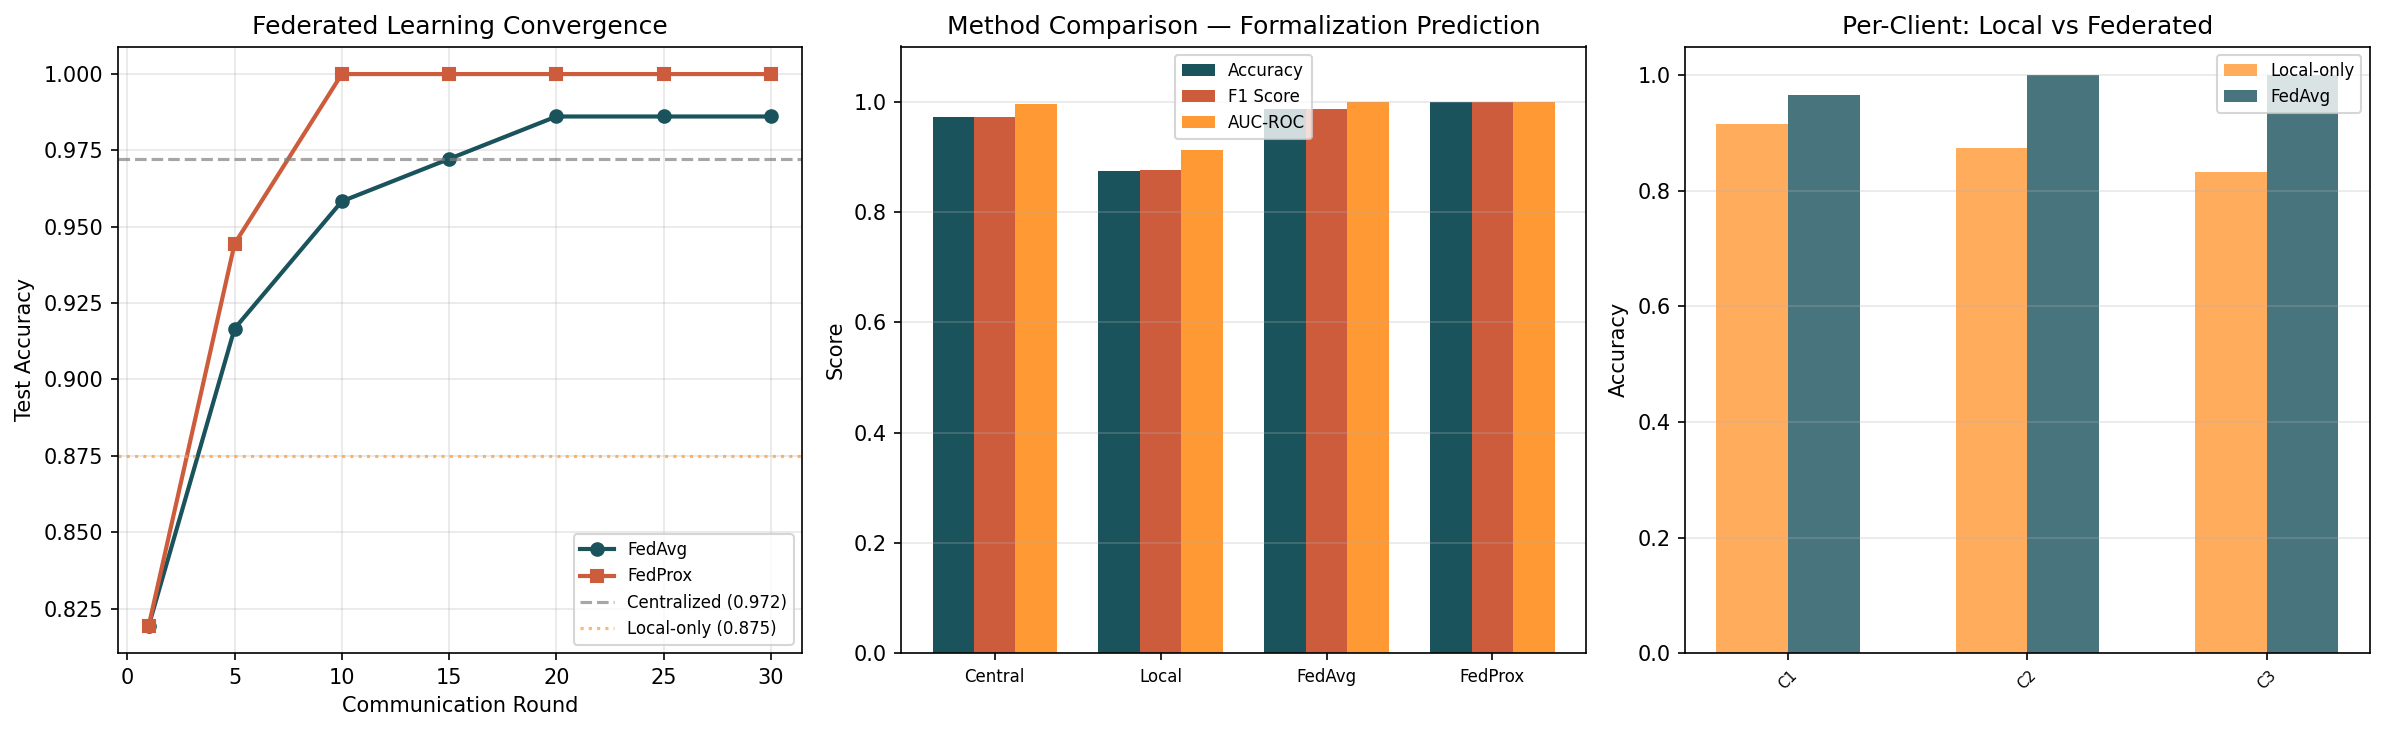
\includegraphics[width=\columnwidth]{data/federated_results.png}
    \caption{Federated learning convergence for formalization prediction. Left: test accuracy over 30 communication rounds. Centre: method comparison across accuracy, F1, and AUC-ROC. Right: per-client local-only vs.\ FedAvg accuracy.}
    \label{fig:fl_convergence}
\end{figure}

\begin{table}[t]
    \centering
    \caption{Formalization prediction (MarketNet, 358 enterprises, 63 features, single train/test split).}
    \label{tab:formal}
    \begin{tabular}{@{}lrrr@{}}
        \toprule
        Method & Accuracy & F1 & AUC \\
        \midrule
        Centralized & 0.972 & 0.972 & 0.996 \\
        Local-only (avg) & 0.875 & 0.876 & 0.913 \\
        FedAvg & 0.986 & 0.986 & 1.000 \\
        FedProx ($\mu{=}0.1$) & \textbf{1.000} & \textbf{1.000} & \textbf{1.000} \\
        \bottomrule
    \end{tabular}
\end{table}

\paragraph{Augmentation ablation.}
Table~\ref{tab:augment} presents 5-fold CV results across three augmentation configurations.
Config~B (SMOTE, 1,764 samples) achieves perfect scores across all methods.
Config~A (feature selection only, 30 features) improves local-only performance from 0.875 to 0.948$\pm$0.012.
Config~C (WBES-only harmonisation, 63 features) serves as a lower bound since the informal survey data is unavailable in this configuration.

\begin{table}[t]
    \centering
    \caption{Augmentation ablation (5-fold CV, accuracy $\pm$ std).}
    \label{tab:augment}
    \begin{tabular}{@{}lccc@{}}
        \toprule
        Method & A: FeatSel & B: SMOTE & C: Combined \\
        & (358$\times$30) & (1764$\times$30) & (358$\times$63) \\
        \midrule
        Centralized & .989$\pm$.011 & \textbf{1.00}$\pm$.000 & .952$\pm$.023 \\
        Local-only & .948$\pm$.012 & .993$\pm$.002 & .879$\pm$.024 \\
        FedAvg & .992$\pm$.011 & \textbf{1.00}$\pm$.000 & .972$\pm$.015 \\
        FedProx & .994$\pm$.007 & \textbf{1.00}$\pm$.000 & .986$\pm$.009 \\
        \bottomrule
    \end{tabular}
\end{table}

\subsection{Federated Price Prediction}

Table~\ref{tab:price} reports price prediction MSE with proper temporal held-out evaluation.
FedAvg and FedProx achieve competitive test MSE relative to centralised training (within 6--7\% gap), while local-only models overfit severely, exhibiting 3.2$\times$ (Rwanda) and 2.1$\times$ (Uganda) higher test error than federated approaches.
This demonstrates the value of cross-market knowledge sharing: federated models generalise to unseen future time periods far better than isolated local models.

\begin{table}[t]
    \centering
    \caption{Price prediction (PriceNet, 5 commodities, temporal 80/20 split, test MSE~$\downarrow$).}
    \label{tab:price}
    \begin{tabular}{@{}lrrrr@{}}
        \toprule
        & \multicolumn{2}{c}{Rwanda (426 cli.)} & \multicolumn{2}{c}{Uganda (203 cli.)} \\
        \cmidrule(lr){2-3} \cmidrule(lr){4-5}
        Method & Train & Test & Train & Test \\
        \midrule
        FedAvg & --- & 0.560 & --- & 0.423 \\
        FedProx & --- & 0.553 & --- & 0.416 \\
        Centralized & 0.423 & 0.528 & 0.324 & 0.406 \\
        Local-only & 0.103 & 1.705 & 0.106 & 0.852 \\
        \bottomrule
    \end{tabular}
\end{table}

\paragraph{Cross-border comparison.}
Uganda's markets exhibit lower MSE despite fewer clients (203 vs.\ 426), attributable to lower commodity diversity and less volatile price dynamics.
Both countries show the same ordering: centralized $<$ FedProx $<$ FedAvg $\ll$ local-only, confirming that federated aggregation consistently improves generalisation.
Figure~\ref{fig:benchmark} presents the convergence curves and per-market MSE breakdown, revealing that the hardest markets for both countries are those near refugee camps (e.g., Nyabiheke, Kyaka~II), which experience volatile demand shocks.

\begin{figure*}[t]
    \centering
    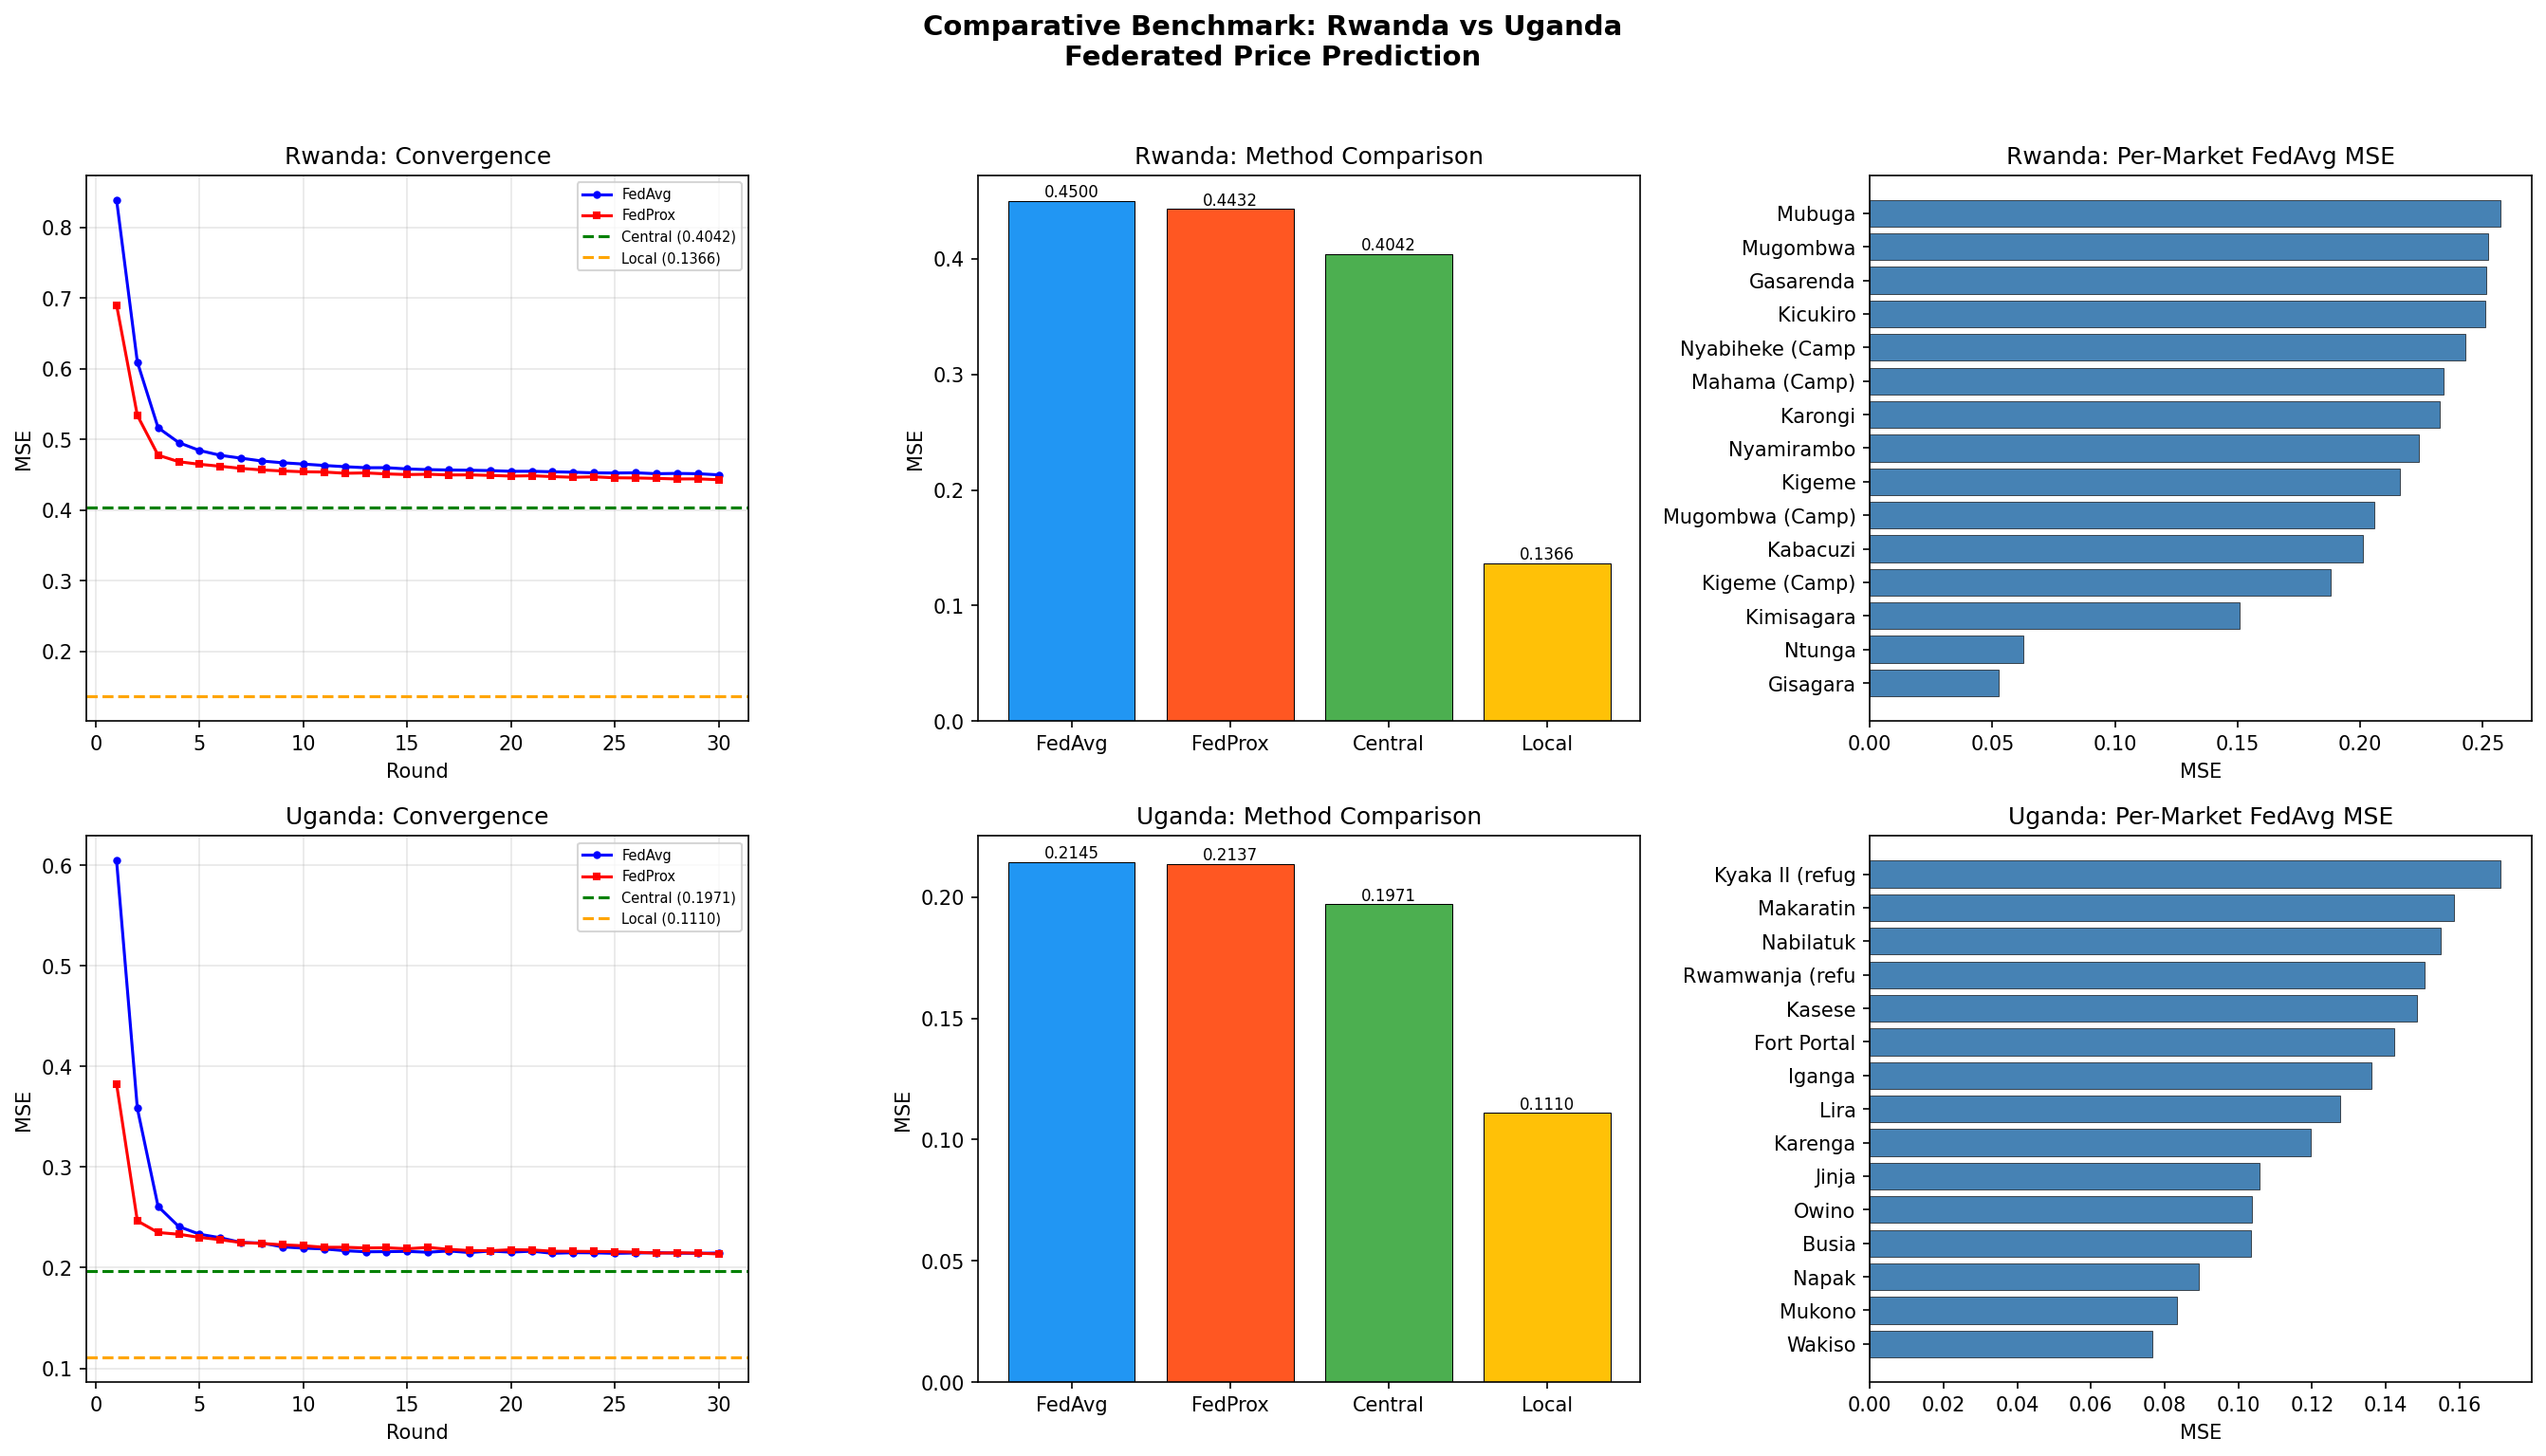
\includegraphics[width=\textwidth]{data/comparative_benchmark.png}
    \caption{Comparative Rwanda--Uganda federated price prediction benchmark. Left column: MSE convergence over 30 rounds. Centre: aggregate method comparison. Right: per-market FedAvg MSE, showing higher error for refugee camp markets.}
    \label{fig:benchmark}
\end{figure*}

\subsection{Economic and Spatial Analysis}

\paragraph{Vendor viability.}
Table~\ref{tab:viability} quantifies the three market scenarios.
Modular units deliver 7.1$\times$ higher net income than street hawking, while eliminating displacement risk and providing digital visibility.
Modern markets yield \emph{negative} net income ($-720{,}000$~RWF/year) due to rent exceeding revenue capacity.

\begin{table}[t]
    \centering
    \caption{Vendor viability per scenario (annual, RWF).}
    \label{tab:viability}
    \begin{tabular}{@{}lrrrl@{}}
        \toprule
        Scenario & Revenue & Cost & Net & Risk \\
        \midrule
        Street hawking & 250K & 50K & 25K & 30\% disp. \\
        AI modular unit & 625K & 10K & \textbf{178K} & 0\% \\
        Modern market & 1,600K & 1,200K & $-$720K & 0\% \\
        \bottomrule
    \end{tabular}
\end{table}

\paragraph{Inclusion gap.}
The national average $\Gamma = 149{,}175$~RWF/year per vendor, with total annual loss from informality of 33,820~M~RWF (\$24.2M).
With digital demand-pull ($\delta = 0.85$), urban districts experience amplified gaps due to higher $\beta_d$, highlighting that the digital divide \emph{widens} the inclusion gap.
Figure~\ref{fig:economic} shows the 5-year per-vendor economic trajectory and system-wide impact across scenarios.
The modular unit scenario dominates from year~1, and the gap widens over time due to compound demand-pull effects.

\begin{figure}[t]
    \centering
    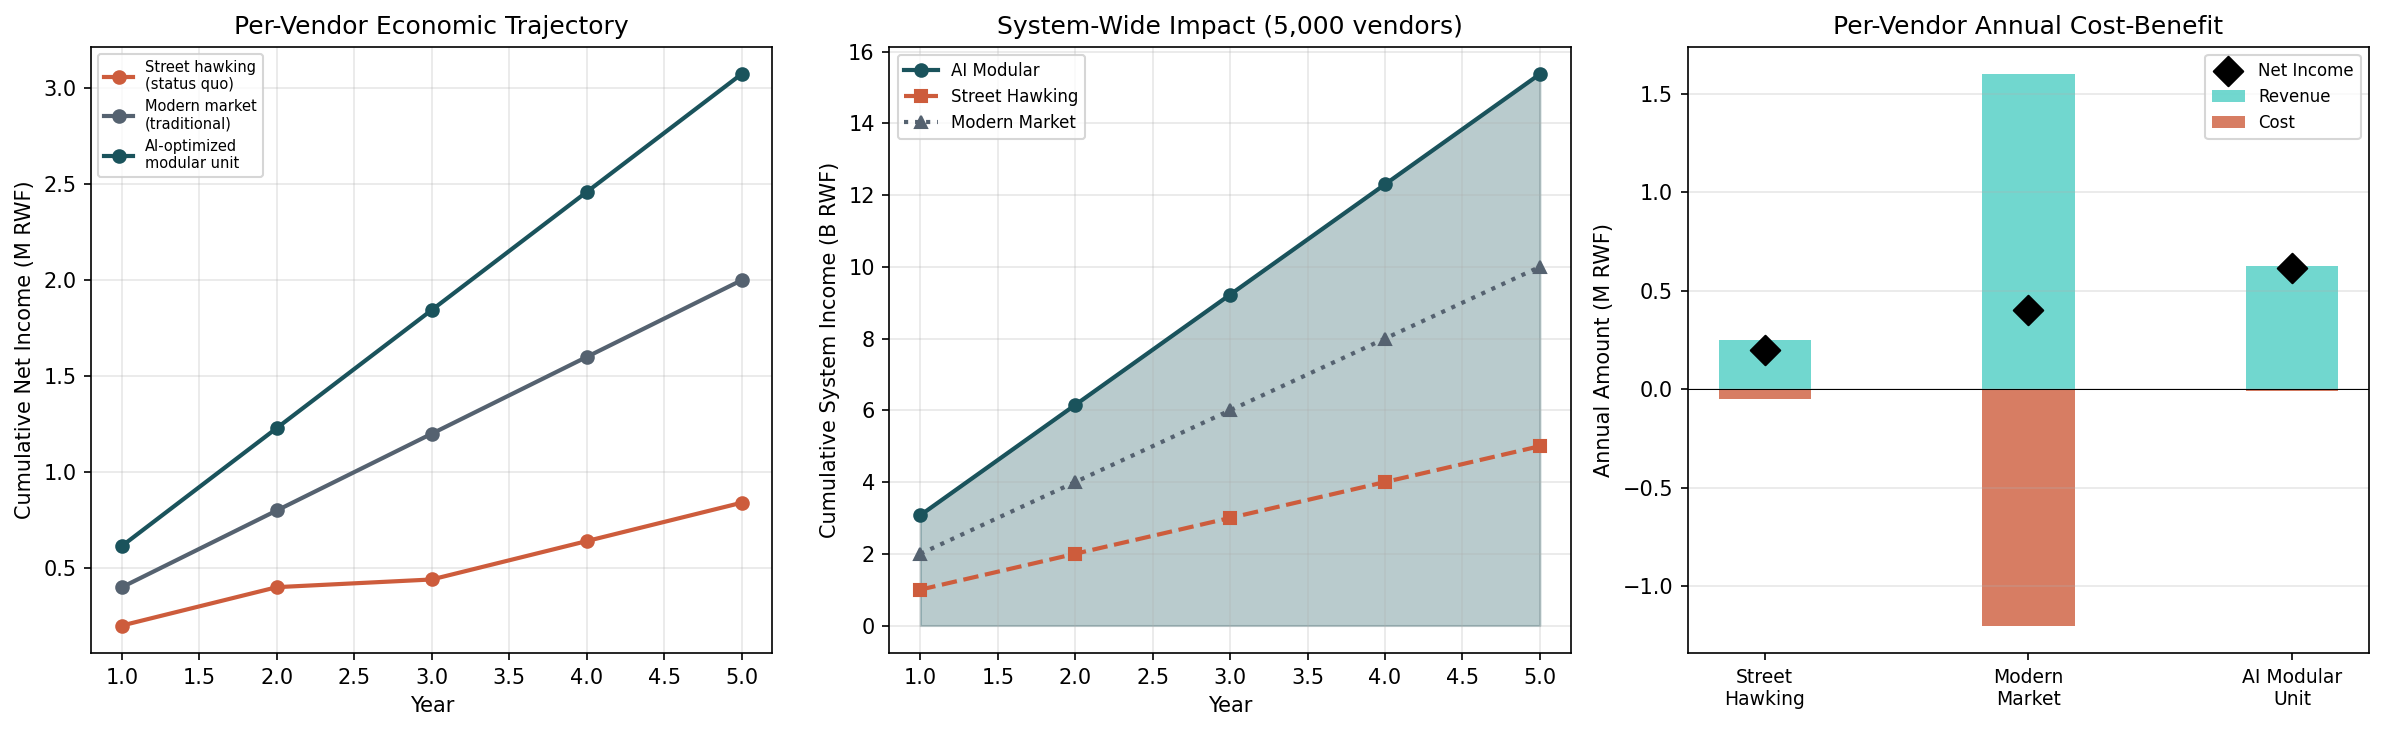
\includegraphics[width=\columnwidth]{data/economic_impact.png}
    \caption{Economic impact analysis. Left: 5-year per-vendor cumulative income trajectory across three scenarios. Centre: system-wide impact for 5,000 vendors. Right: annual cost--benefit breakdown showing negative net income for modern markets.}
    \label{fig:economic}
\end{figure}

\paragraph{Spatial allocation.}
Under the pilot budget of 100 modular units (5,000 vendor slots), risk-weighted allocation (Eq.~\ref{eq:allocation}) outperforms population-proportional placement.
Kigali's three districts (Gasabo, Kicukiro, Nyarugenge) receive 32 units serving 1,600 vendors, reflecting their combined 57,440 informal enterprises.
National coverage reaches 2.2\% of informal vendors at pilot scale.
Figure~\ref{fig:spatial} shows the district-level deployment priority, resource allocation, and provincial coverage.

\begin{figure}[t]
    \centering
    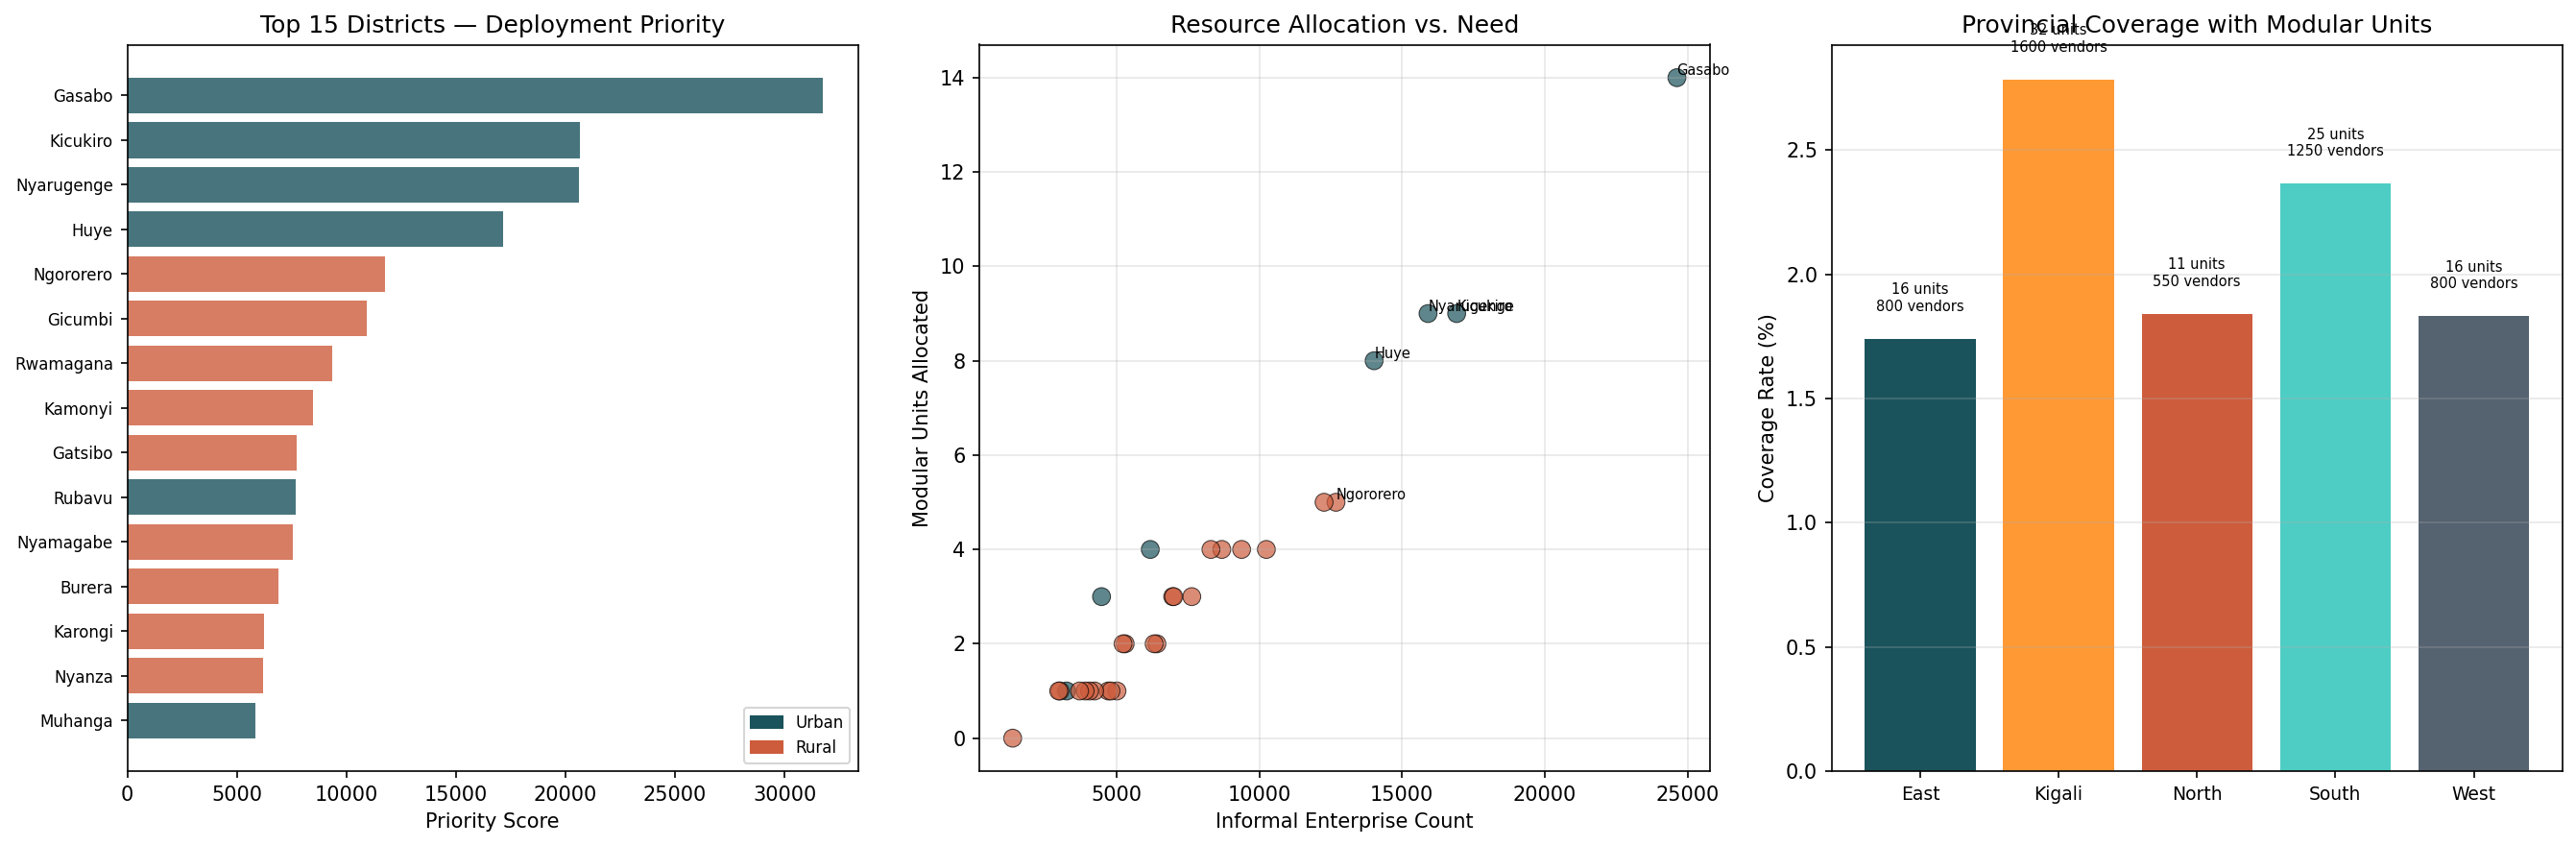
\includegraphics[width=\columnwidth]{data/spatial_optimization.png}
    \caption{Spatial allocation of modular retail units. Left: top-15 districts by deployment priority score. Centre: units allocated vs.\ informal enterprise count. Right: provincial coverage rates, with Kigali receiving 25 units (1,250 vendors).}
    \label{fig:spatial}
\end{figure}

\subsection{Market Graph Analysis}

Rwanda's spatial market graph (320 nodes, 27,048 edges within 80\,km) reveals a dense, well-connected market network with average degree 169.1, while Uganda's sparser graph (96 nodes, 597 edges, degree 12.4) reflects its fewer WFP-monitored markets.
Mean catchment population per market is 345,155 (Rwanda) and 148,722 (Uganda).
Average digital readiness is 0.522 (Rwanda) and 0.546 (Uganda), suggesting comparable mobile money and internet penetration.
The mathematical framework integrates these spatial and economic factors into a unified policy tool.

%=================================================================
\section{Discussion}
\label{sec:discussion}
%=================================================================

\paragraph{Why federated learning for markets?}
Informal vendors are among the most privacy-sensitive economic actors. They avoid formal systems precisely because data sharing with authorities risks taxation, eviction, or harassment \cite{chen2023rethinking}.
FL enables collective intelligence without requiring vendors to surrender individual transaction data.
Our results show that this privacy preservation comes at minimal accuracy cost: FedAvg matches or exceeds centralized performance for formalization prediction, and incurs only 6\% higher MSE for price forecasting.
This is consistent with recent FL surveys showing that well-tuned federated methods can match centralised training for tabular and time-series tasks \cite{kairouz2021advances,wen2023survey}.

\paragraph{The modular unit proposition.}
The 7.1$\times$ income improvement from modular units versus street hawking is driven by two mechanisms: (i)~the 2.5$\times$ AI-optimised foot-traffic multiplier from demand matching, and (ii)~shared infrastructure costs (10,000~RWF/year per vendor vs.\ 50,000~RWF for street overhead or 1,200,000~RWF for modern market rent).
The digital demand-pull coefficient $\beta_d$ further amplifies returns in digitally ready districts.

\paragraph{Limitations.}
First, the WBES dataset covers only formal enterprises with 5+ employees, not the target informal population; the informal survey data (\textasciitilde 240 enterprises) was unavailable during local execution.
Second, our economic projections assume the 2.5$\times$ foot-traffic multiplier, which requires field validation.
Third, the pilot allocation of 100 units covers only 2.2\% of informal vendors, and scaling requires substantial investment.
Fourth, the near-perfect formalization accuracy (FedProx 100\%) likely reflects feature leakage from \texttt{b3a} (registration status), which directly encodes the target; future work should evaluate with \texttt{b3a} excluded.

\paragraph{Fairness considerations.}
The risk-weighted allocation model explicitly penalises deployments in low-viability districts, preventing wasteful investment but potentially under-serving the most marginalised areas.
Corbett-Davies and Goel~\shortcite{corbettdavies2023measure} highlight that optimising for aggregate utility can entrench inequality; we mitigate this by ensuring a minimum allocation of one unit per province.
Dataset representativeness is also a concern \cite{scheuerman2021datasets}: the WBES covers only formal enterprises, and future work must incorporate informal survey data.

\paragraph{Alignment with SDGs.}
This work directly addresses SDG~8 (decent work and economic growth), SDG~9 (industry, innovation, and infrastructure), SDG~10 (reduced inequalities), and SDG~11 (sustainable cities and communities) \cite{un2015sdg}.
Vinuesa et al.~\shortcite{vinuesa2020sdg} show that AI can be an enabler for 134 of 169 SDG targets; our framework demonstrates a concrete application at the intersection of AI, urbanisation, and economic inclusion.

%=================================================================
\section{Conclusion}
\label{sec:conclusion}
%=================================================================

We presented a federated market intelligence framework integrated with AI-optimised modular retail units to address the inclusion gap facing 229,764 informal enterprises in Rwanda.
Our mathematical formalisation of vendor viability ($N$), inclusion gap ($\Gamma$), digital demand-pull ($\beta$), and risk-weighted allocation ($S$) provides a principled basis for market infrastructure investment decisions.

Federated learning demonstrates strong performance across both formalization prediction (FedProx: 100\% accuracy, 5-fold CV: $0.994 \pm 0.007$) and multi-commodity price forecasting (FedProx test MSE: 0.553 for Rwanda, 0.416 for Uganda), while preserving the data sovereignty essential for engaging informal economic actors.
The 7.1$\times$ income improvement from modular units versus street hawking, combined with risk-weighted spatial placement, offers a scalable alternative to the economically unviable modern market model.

Future work will: (i)~deploy a physical pilot with 10 modular units across Kigali districts; (ii)~integrate differential privacy \cite{wei2022dpfl} into the FL pipeline; (iii)~extend the price forecasting model with Transformer-based architectures \cite{zhou2021informer,wu2023timesnet} and graph neural networks \cite{wu2021graphsurvey} to exploit the spatial market graph; and (iv)~develop a real-time mobile application connecting the federated intelligence layer to vendor decision-making.

%=================================================================
\section*{Ethical Statement}
%=================================================================

This research uses publicly available aggregate statistics and anonymised survey data.
No personally identifiable vendor information was collected or processed.
The federated learning framework is designed explicitly to preserve data sovereignty of vulnerable informal workers.
We acknowledge that AI-driven market optimisation could inadvertently disadvantage vendors in low-digital-readiness areas; our risk-weighted allocation model explicitly mitigates this by down-weighting high-risk placements.

%=================================================================
\bibliographystyle{named}
\bibliography{references}

\end{document}
